\section{Řízení operační paměti}

Řízení operační paměti je klíčovým aspektem operačních systémů, které zajišťuje efektivní správu a využití paměti počítače. Správné řízení paměti umožňuje více procesům sdílet paměťový prostor bez konfliktů a zajišťuje, že každý proces má dostatek paměti pro svůj běh.

\subsection{Operační paměť}

Operační paměť, známá také jako RAM (Random Access Memory), je hlavní úložiště, které procesor využívá k dočasnému ukládání a přístupu k datům a instrukcím, které jsou aktuálně ve zpracování. Na rozdíl od sekundární paměti (např. pevný disk) je operační paměť rychlá a umožňuje přímý přístup k libovolným místům, což je zásadní pro efektivní běh aplikací a systémů.

\subsection{Strategie přidělování operační paměti}

Existuje několik strategií přidělování operační paměti, které zajišťují efektivní využití dostupného paměťového prostoru:

\paragraph{Souvislá oblast}
Přidělování po blocích rozděluje paměť do dvou hlavních částí, a to:
\begin{itemize}
    \item Část pro operační systém.
    \item Část pro uživatelský program.
\end{itemize}

\begin{figure}[h]
    \centering
    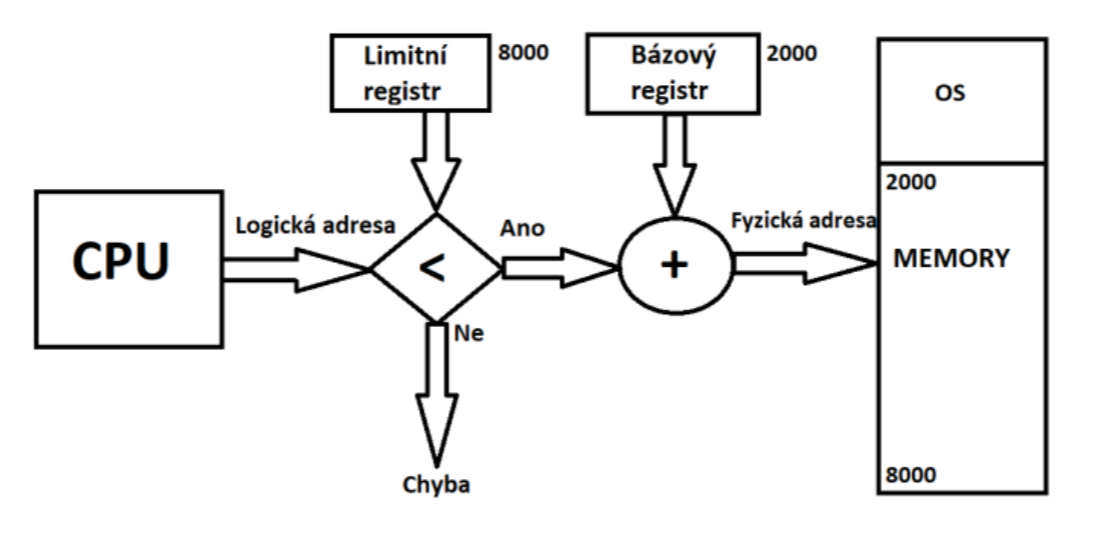
\includegraphics[scale=0.3]{sections/8_riz_op_pam/images/Screenshot 2024-08-26 121515.png}
 
\end{figure}
Nevýhodou je, že není využita celá paměť, výhodou je jednoduchost. Pokud je proces větší než je místo v OP, je možné to řešit prokládáním = Proces je rozdělen na 2 částí, a to na: Část která musí být neustále v OP a část která tam být nemusí.

\paragraph{Po blocích}
Kromě OS se v paměti může nacházet více než 1 proces. Paměť je rozdělena na bloky (sekce) o stejné velikosti. Nutnost dopředu znát velikost úlohy. Používá alokační strategie: first fit, last fit, best fit, worst fit. Příklad: MS DOS

\paragraph{Stránkování}
Stránkování je technika, která rozděluje paměť na malé, pevně velké stránky/rámce. Operační systém udržuje tabulky stránek, které mapují virtuální adresy na fyzické adresy. Tato metoda eliminuje externí fragmentaci a umožňuje efektivní využití paměti, ale vyžaduje správu tabulek stránek.

\begin{figure}[h]
    \centering
    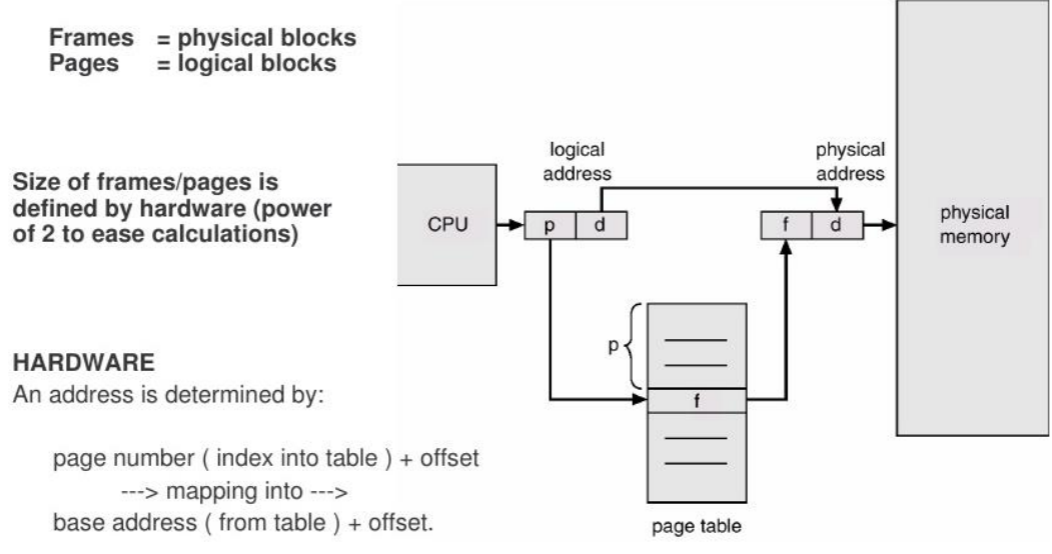
\includegraphics[scale=0.3]{sections/8_riz_op_pam/images/Screenshot 2024-08-26 125926.png}

\end{figure}

\paragraph{Segmentace}
Segmentace proces na segmenty různé velikosti podle logické struktury programu, jako jsou kód, data a zásobník. Každý segment má svou vlastní základní adresu a limit. Tento přístup umožňuje lepší organizaci paměti a ochranu, ale může vést k fragmentaci.

\begin{figure}[h]
    \centering
    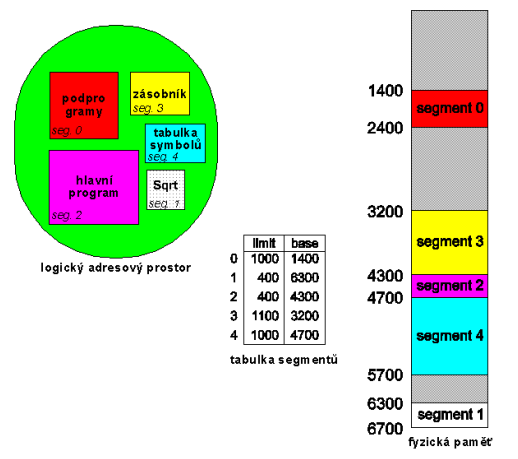
\includegraphics[scale=0.3]{sections/8_riz_op_pam/images/Screenshot 2024-08-26 130622.png}

\end{figure}

\paragraph{Segmentace se stránkováním}
Kombinace segmentace a stránkování využívá výhod obou metod. Paměť je rozdělena na segmenty, které jsou dále rozděleny na stránky. Tento přístup zajišťuje flexibilitu segmentace a efektivitu stránkování, čímž minimalizuje fragmentaci a zvyšuje ochranu paměti.

\begin{figure}[h]
    \centering
    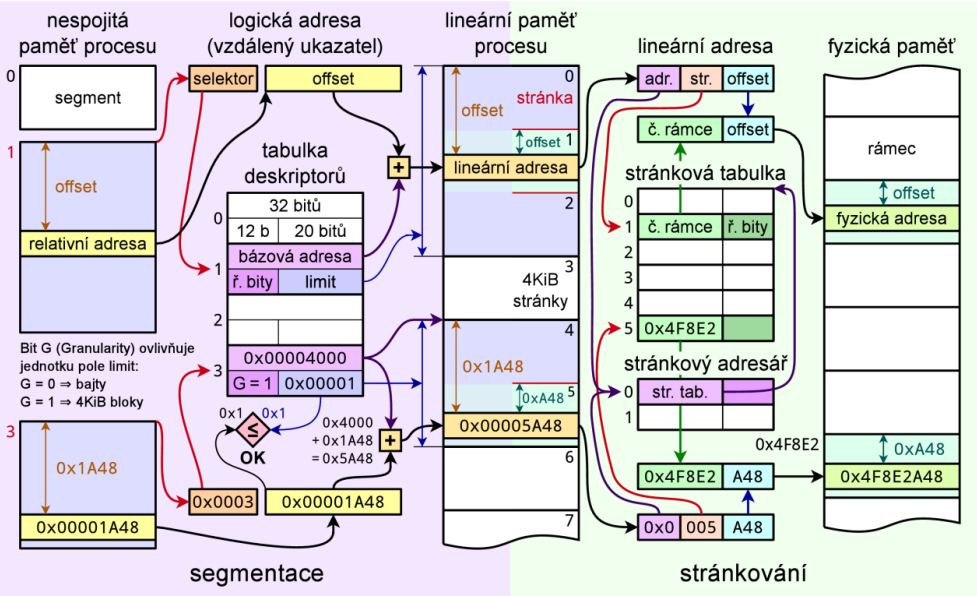
\includegraphics[scale=0.3]{sections/8_riz_op_pam/images/Screenshot 2024-08-26 130536.png}
\end{figure}

\subsection{Výpadek stránky, pre-cleaning, thrashing}

\paragraph{Výpadek stránky}
Výpadek stránky nastává, když proces žádá o stránku, která není v hlavní paměti (RAM), a musí být načtena ze sekundární paměti (např. pevný disk). To způsobuje zpoždění, protože přístup k disku je pomalejší než přístup k RAM.

\paragraph{Pre-cleaning}
Pre-cleaning je technika, která předem zapisuje špinavé stránky (stránky, které byly modifikovány) zpět do sekundární paměti před jejich skutečným vyřazením. Tím se snižuje zpoždění způsobené výpadky stránek, protože stránky jsou již připraveny k výměně.

\paragraph{Thrashing}
Thrashing nastává, když systém tráví více času výměnou stránek mezi hlavní a sekundární pamětí než vykonáváním užitečné práce. To se obvykle stává, když není dostatek paměti pro všechny běžící procesy, což vede k neustálým výpadkům stránek.

\subsection{Čisté a špinavé stránky}

\paragraph{Čisté stránky}
Čisté stránky jsou ty, které nebyly modifikovány od doby, kdy byly načteny do paměti nebo od posledního zápisu na disk. Jejich vyřazení z paměti je jednoduché, protože není nutné je zapisovat zpět na disk.

\paragraph{Špinavé stránky}
Špinavé stránky jsou ty, které byly modifikovány od doby, kdy byly načteny do paměti. Před jejich vyřazením z paměti je nutné je zapsat zpět na disk, aby se uchovaly změny.

\subsection{Algoritmy výměny stránek}

Různé algoritmy výměny stránek se používají k rozhodování, které stránky mají být vyřazeny z paměti, když je potřeba uvolnit místo pro nové stránky. Každý algoritmus má své výhody a nevýhody v různých scénářích.

\paragraph{Optimální}
Optimální algoritmus (OPT) vyřazuje stránku, která nebude potřebná pro nejdelší dobu v budoucnosti. Tento algoritmus poskytuje nejlepší možný výkon, ale je teoretický, protože budoucí přístupy nejsou předem známy.

\paragraph{FIFO}
FIFO (First-In, First-Out) algoritmus vyřazuje stránku, která byla v paměti nejdéle. Tento přístup je jednoduchý, ale může vést k špatnému výkonu, protože nejstarší stránka nemusí být ta nejméně potřebná.

\paragraph{LRU}
LRU (Least Recently Used) algoritmus vyřazuje stránku, která nebyla nejdéle používána. Tento přístup je účinný, protože stránky, které nebyly dlouho používány, jsou pravděpodobně méně potřebné, ale vyžaduje sledování historie přístupů.

\paragraph{Druhá šance}
Druhá šance je vylepšení FIFO, které poskytuje stránkám druhou šanci, pokud byly nedávno použity. Když je stránka určena k vyřazení, kontroluje se její stav; pokud byla nedávno použita, dostane další šanci a algoritmus pokračuje k další stránce.

\paragraph{Hodiny}
Hodinový algoritmus je implementace druhé šance, kde stránky jsou uspořádány do kruhu a kontrolují se jako hodinové ručičky. Stránky, které nebyly nedávno použity, jsou vyřazeny, což poskytuje jednoduchou a efektivní správu paměti.

\paragraph{NUR/NRU}
NUR (Not Used Recently) nebo NRU (Not Recently Used) algoritmus klasifikuje stránky do čtyř kategorií na základě jejich nedávného použití a modifikace. Stránky v nejnižší kategorii jsou vyřazeny jako první. Tento algoritmus je jednodušší než LRU, ale poskytuje dobrý výkon.

\paragraph{Random}
Náhodný algoritmus vybere stránku k vyřazení náhodně. I když je tento přístup jednoduchý a nevyžaduje žádné sledování, jeho výkon může být nekonzistentní a často horší než jiné algoritmy.

\paragraph{NFU}
NFU (Not Frequently Used) algoritmus sleduje počet přístupů ke každé stránce a vyřazuje stránku s nejnižším počtem přístupů. Tento přístup se podobá LRU, ale místo nedávného použití sleduje celkovou frekvenci přístupů. Nevýhodou je, že stránky, které byly často používány v minulosti, ale již nejsou, mohou zůstat v paměti déle, než je potřeba.







